\section{Calibration analysis on synthesis data}

\subsection{Data}

Approximating calibration statistics is very difficult since the distribution of the true labels is unknown. Therefore, we investigate the behavior of calibration statistics on synthesized set of prediction-observation pairs that mimics common NLP data distributions. 

Each prediction-observation pair is generated as follows. First of all, the value of the prediction is drawn from a beta distribution. Then, the observation is obtained by sampling from a Bernoulli distribution whose parameter is a transformation of the value of the prediction. To obtain a perfectly calibrated set of pairs, we use the identity transformation. For uncalibrated condition, we use this function $t(p)$:

\[
        t(p) =
\begin{cases}
  \max(0, p - k), & \text{if } 0 \leq x \leq 0.5 \\
  \min(0, p + k), & \text{otherwise}
\end{cases}
\]
where k $\in$ [0, 0.5].

\begin{figure}[t]
\minipage{0.5\textwidth}
  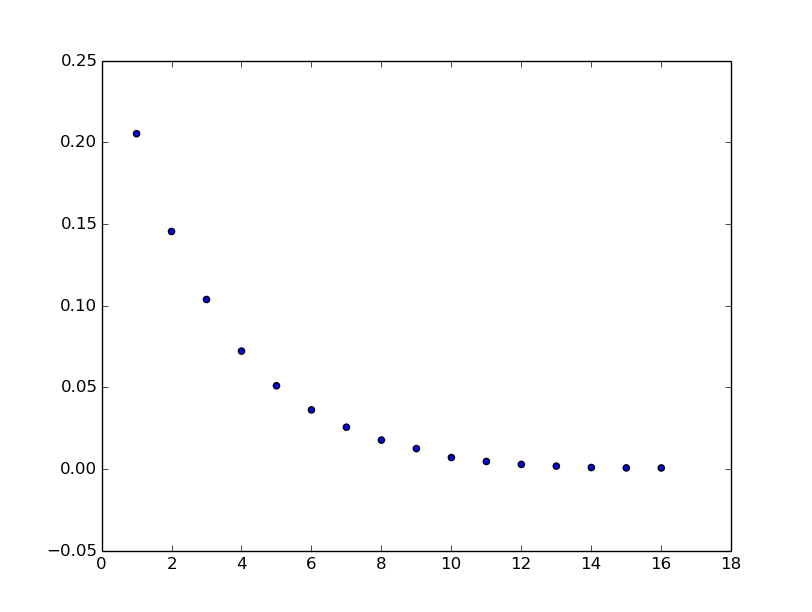
\includegraphics[width=\linewidth]{calibrated_binsize_score_log_scale.png}
  \caption{MSE calibration score versus bin size (Log scale) for calibrated predictions}
  \label{fig:binsize_score_calib_log}
\endminipage\hfill
\minipage{0.5\textwidth}
  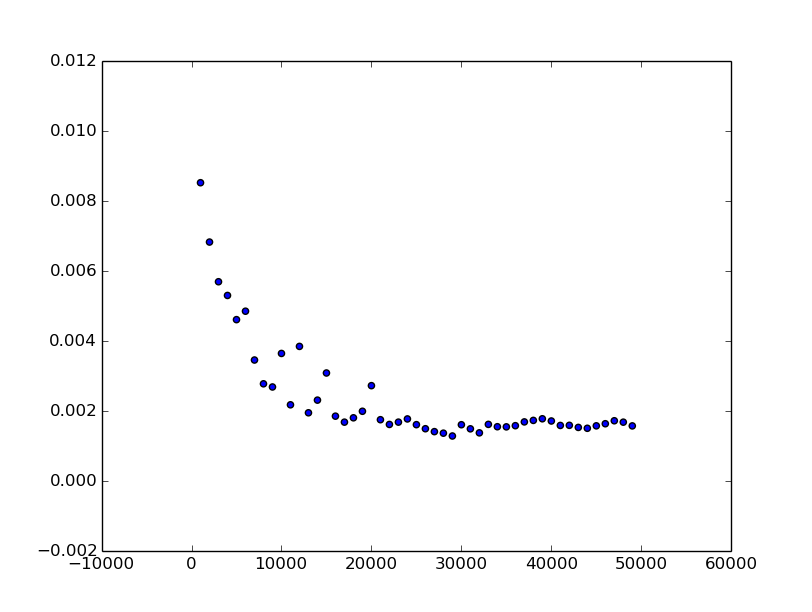
\includegraphics[width=\linewidth]{calibrated_binsize_score.png}
  \caption{MSE calibration score versus bin size for calibrated predictions}
  \label{fig:binsize_score_calib}
\endminipage\hfill
\minipage{0.5\textwidth}
  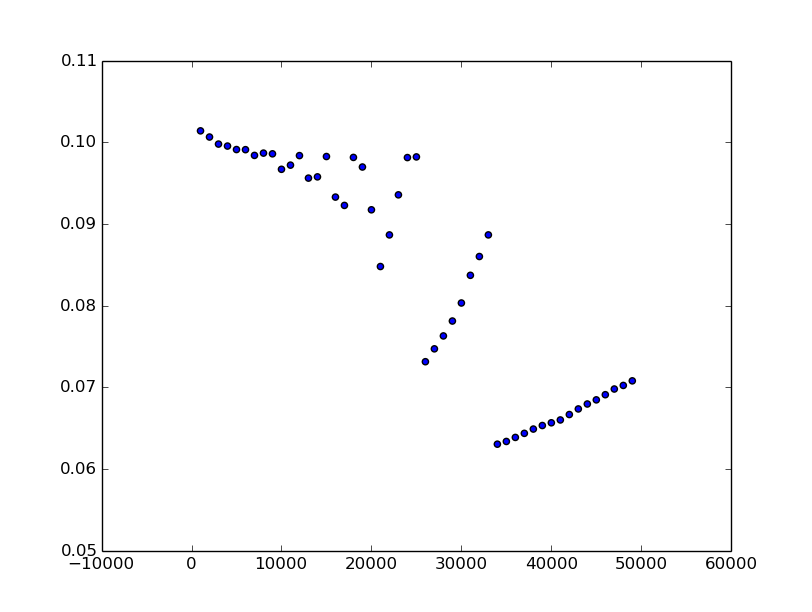
\includegraphics[width=\linewidth]{uncalibrated_binsize_score.png}
  \caption{MSE calibration score versus bin size for uncalibrated predictions}
  \label{fig:binsize_score_uncalib}
\endminipage
\end{figure}


\subsection{Effect of bin size on calibration score}

\begin{figure}[t]
\minipage{0.5\textwidth}
  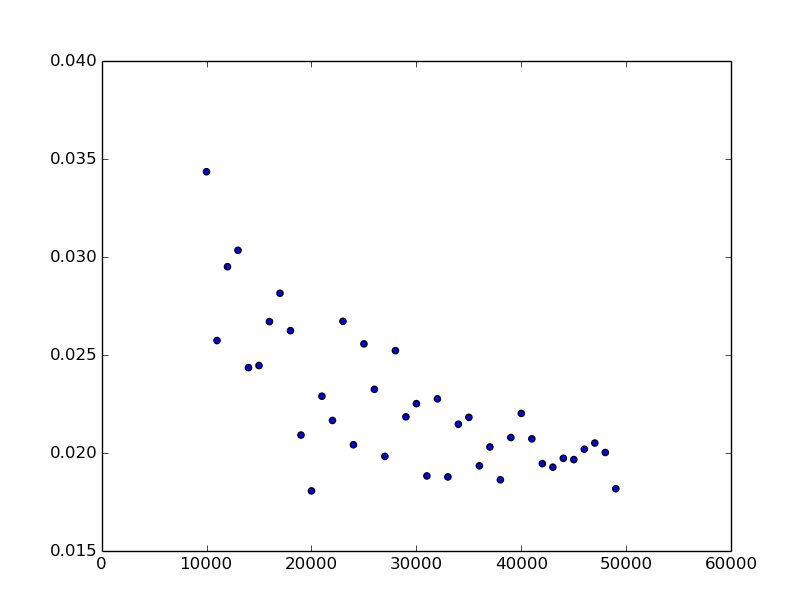
\includegraphics[width=\linewidth]{calibrated_sampleSize_score.png}
  \caption{MSE calibration score versus sample size for calibrated predictions}
  \label{fig:calibrated_samplesize_score}
\endminipage\hfill
\minipage{0.5\textwidth}
  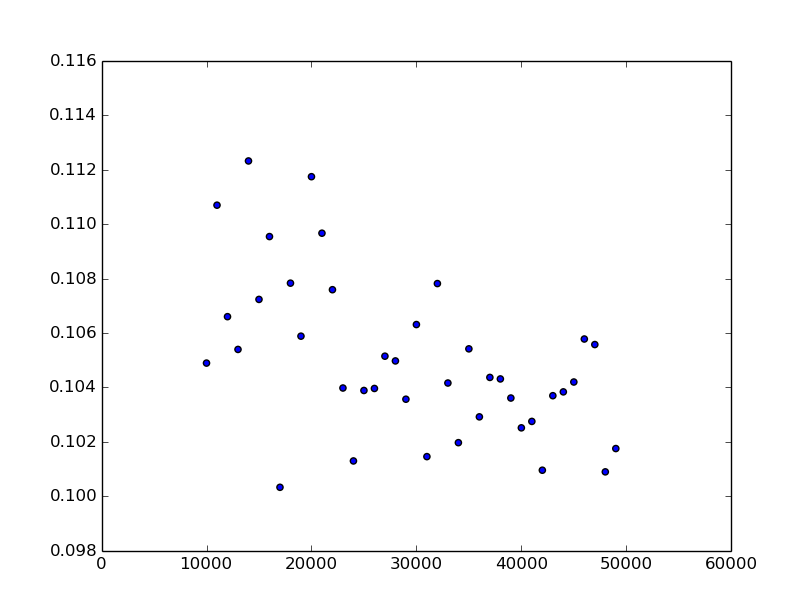
\includegraphics[width=\linewidth]{uncalibrated_sampleSize_score.png}
  \caption{MSE calibration score versus sample size for uncalibrated predictions}
  \label{fig:uncalibrated_samplesize_score}  
\endminipage
\end{figure}

We investigate the the effect of varying the bin size on the value of the MSE calibration score. Theoretically, as we double the bin size, the score will not increase. This fact is obtain by using Jensen's inequality, leveraging the fact that the quaratic function is convex. In our experiment, we vary the bin size from $2^1$ to $2^16$ to calculate the MSE calibration score on a data set consists of $10^5$ pairs. Our result (Figure BLAH BLAH) supports the theoretical hypothesis. The score monotonically decreases as the bin size exponentally increases. We also alter the parameters of our beta distribution and witness the same pattern. We attempt to generalize this pattern to a contious range of bin size values. Figure BLAH BLAH portrays the behavior of the score of a perfectly calibrated predictor as the bin size goes from $10^3$ to $5.10^4$ with a step size of $10^3$. As we can see, although the points do not always monotonically decrease, we see a similiar trend as the log-scale plot. However, for an uncalibrated predictor, the score is much more unpredictable (Figure BLAH BLAH). 

\subsection{Effect of sample size on calibration score}

As pointed out by Foster (1998), we expect the calibration score of a perfectly calibrated predictor to go to zero as the sample size goes to infinity. We set up experiment to verify this fact. Using a range of sample size from $10^4$ to $5.10^4$, we compute the calibration score for three set of predictions: perfectly calibrated (PERFECT), uncalibrated using the function t(p) as true distribution with k = 0.1 (UNCALIB). For each experiement, we set the bin size to be the square root of the sample size. We observed distinguishing pattern between PERFECT and UNCALIB. The points in the CALIB's plot clearly approach zero while those of the UNCALIB's plot converge weakly. 


